% !TeX root = ../thuthesis-example.tex

\chapter{系统框架与离线建图}

本章主要对系统框架和离线建图模块进行介绍。在系统框架介绍部分展示了整体设计、信息输入以及3个子模块关系,同时为了方便后文详细介绍子模块,还进行了坐标系的统一介绍。在离线建图模块介绍部分展示了该模块的基本运行过程,详细介绍了各个过程的设计目和实际功能。

\section{系统框架}

本文所提出方法的整体设计如图\ref{fig:overall}所示,其主要包括两个阶段:建图和定位。在建图阶段,离线建图模块使用图片和高精度GNSS信息构建包含粗粒度和细粒度信息的先验地图。在定位阶段又可以分为两个模块:视觉惯性里程计模块和紧耦合地图定位模块。

视觉惯性里程计使用图片和惯性信息可以获得连续图片的相对位姿变换;紧耦合地图定位则VIO结果和地图观测完成最后的定位,获得相机位姿。整个系统的设计与研究内容的对应关系是:离线建图模块对应着先验地图构建的研究内容,将在本章着重介绍;VIO对应着视觉与惯性信息的融合的研究内容,将在第3章中着重介绍;紧耦合地图定位对应着基于先验地图的位姿优化的研究内容,将在第4章中着重介绍。

\begin{figure}
  \centering
  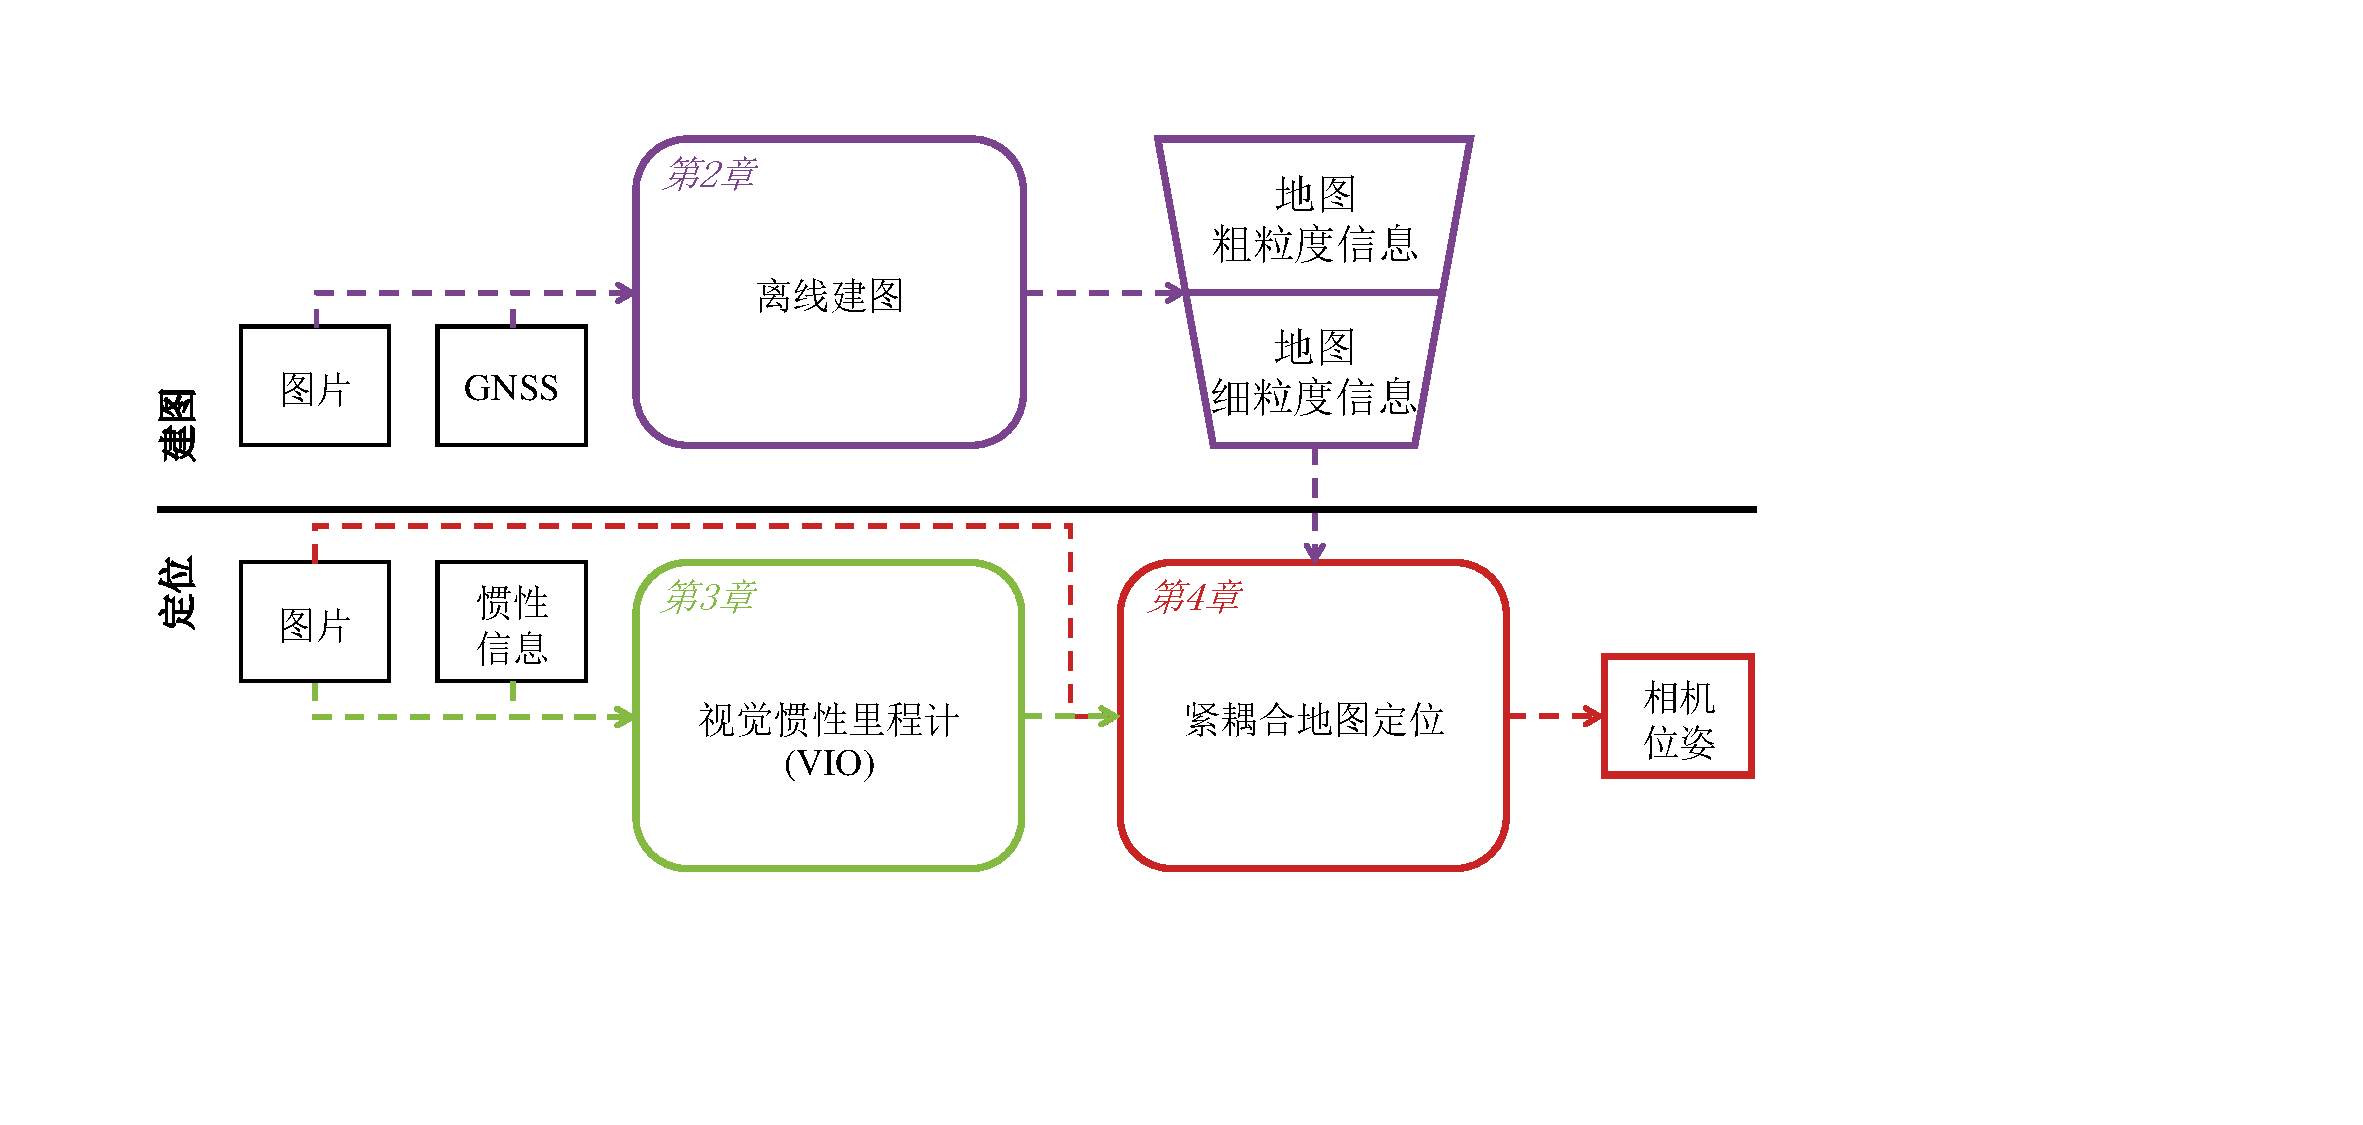
\includegraphics[width=1.0\linewidth]{overall.pdf}
  \caption{系统框架的设计示意图}
  \label{fig:overall}
\end{figure}

建图阶段,离线建图模块利用GNSS观测数据和图像构建一个包含粗粒度层级和细粒度层级组成的分层先验地图。粗粒度层级包括地图关键帧的位姿和关键帧描述子,而细粒度层级则包含稀疏点云结构及点云点描述子。添加GNSS观测的SfM是离线建图模块的核心,使用这一技术有以下的必要性:首先,SfM作为一种具有全局优化功能的建图方式,其相较于SLAM更适合建立高精度的地图;其次,SfM作为一种单目建图技术,其所创建的地图并不具有真实物理世界的尺度,因此必须添加具有尺度信息的GNSS信息作为补充,以获得具有真实世界尺度的地图;最后,相对精确的GNSS信息对于SfM的建图过程也有增益,有助于获得更加精确的地图。

基于建图阶段所构建的分层先验地图,视觉惯性里程计模块和紧耦合地图定位模块计算实际定位时所拍摄图像在全局坐标系中的位姿。

在视觉惯性里程计模块中,图像和惯性信息经过融合后可以相对精确地估算相邻图片之间的位姿变换,虽然这种相对信息虽然不是绝对的全局位姿,不可以直接用来作为定位结果,但是可以作为约束条件用于实际的地图定位。作为一种约束条件,视觉惯性里程计的精度对于整个定位系统的性能也发挥着重要作用,因此,本文将提升视觉里程计的精度也作为一项重要研究内容。

紧耦合定位模块是整个系统最后,也是最重要的模块,其主要功能包括地图观测与定位、视觉惯性里程计对齐、紧耦合位姿优化等。地图的观测与定位将实际拍摄的图片与地图进行粗到细匹配,逐渐获得一个较为粗糙的位姿观测;视觉惯性里程计对齐则将视觉惯性里程计的相对位姿转化到地图坐标系中,方便其后续使用;紧耦合位姿优化是整个模块的核心,其同时参考视觉惯性里程计、地图观测以及地图先验信息,通过非线性优化算法获得最终的精确位姿。

\begin{figure}
  \centering
  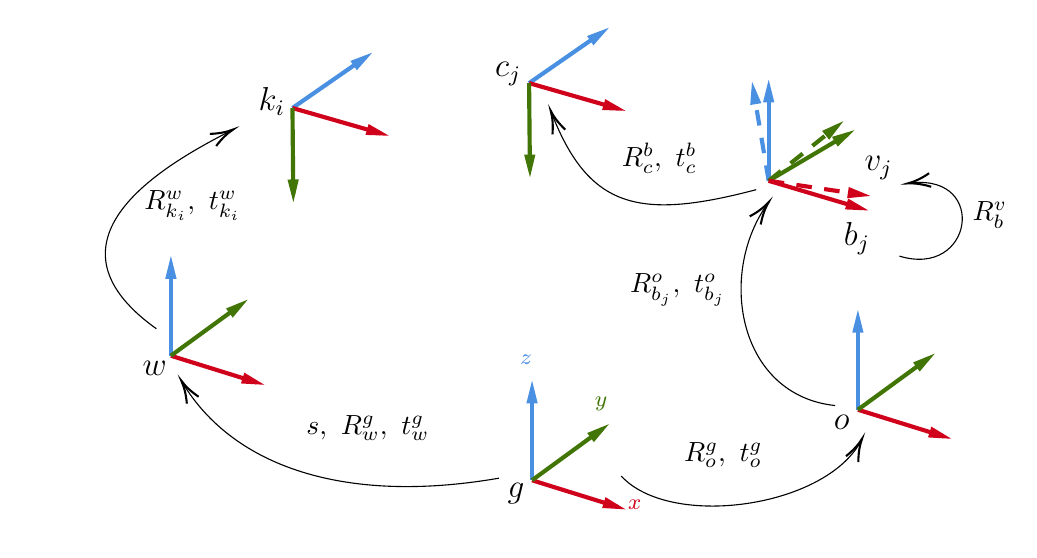
\begin{tikzpicture}[x=0.75pt,y=0.75pt,yscale=-1,xscale=1]
    %uncomment if require: \path (0,381); %set diagram left start at 0, and has height of 381
    
    %Straight Lines [id:da010349331460429267] 
    \draw [color={rgb, 255:red, 74; green, 144; blue, 226 }  ,draw opacity=1 ][line width=1.5]    (405,86.72) -- (405,42) ;
    \draw [shift={(405,38)}, rotate = 90] [fill={rgb, 255:red, 74; green, 144; blue, 226 }  ,fill opacity=1 ][line width=0.08]  [draw opacity=0] (10.92,-2.73) -- (0,0) -- (10.92,2.73) -- cycle    ;
    %Straight Lines [id:da02660288208799133] 
    \draw [color={rgb, 255:red, 208; green, 2; blue, 27 }  ,draw opacity=1 ][line width=1.5]    (405,86.72) -- (449.17,99.86) ;
    \draw [shift={(453,101)}, rotate = 196.57] [fill={rgb, 255:red, 208; green, 2; blue, 27 }  ,fill opacity=1 ][line width=0.08]  [draw opacity=0] (10.92,-2.73) -- (0,0) -- (10.92,2.73) -- cycle    ;
    %Straight Lines [id:da6739104782471683] 
    \draw [color={rgb, 255:red, 65; green, 117; blue, 5 }  ,draw opacity=1 ][line width=1.5]    (405,86.72) -- (442.86,64.39) ;
    \draw [shift={(446.3,62.36)}, rotate = 149.47] [fill={rgb, 255:red, 65; green, 117; blue, 5 }  ,fill opacity=1 ][line width=0.08]  [draw opacity=0] (10.92,-2.73) -- (0,0) -- (10.92,2.73) -- cycle    ;
    %Straight Lines [id:da8429448182305654] 
    \draw [color={rgb, 255:red, 74; green, 144; blue, 226 }  ,draw opacity=1 ][line width=1.5]  [dash pattern={on 5.63pt off 4.5pt}]  (405,86.72) -- (397.66,42.94) ;
    \draw [shift={(397,39)}, rotate = 80.48] [fill={rgb, 255:red, 74; green, 144; blue, 226 }  ,fill opacity=1 ][line width=0.08]  [draw opacity=0] (10.92,-2.73) -- (0,0) -- (10.92,2.73) -- cycle    ;
    %Straight Lines [id:da4153681450236333] 
    \draw [color={rgb, 255:red, 65; green, 117; blue, 5 }  ,draw opacity=1 ][line width=1.5]  [dash pattern={on 5.63pt off 4.5pt}]  (405,86.72) -- (437.87,60.49) ;
    \draw [shift={(441,58)}, rotate = 141.42] [fill={rgb, 255:red, 65; green, 117; blue, 5 }  ,fill opacity=1 ][line width=0.08]  [draw opacity=0] (10.92,-2.73) -- (0,0) -- (10.92,2.73) -- cycle    ;
    %Straight Lines [id:da43505559959247075] 
    \draw [color={rgb, 255:red, 208; green, 2; blue, 27 }  ,draw opacity=1 ][line width=1.5]  [dash pattern={on 5.63pt off 4.5pt}]  (405,86.72) -- (450.04,93.41) ;
    \draw [shift={(454,94)}, rotate = 188.45] [fill={rgb, 255:red, 208; green, 2; blue, 27 }  ,fill opacity=1 ][line width=0.08]  [draw opacity=0] (10.92,-2.73) -- (0,0) -- (10.92,2.73) -- cycle    ;
    %Straight Lines [id:da48780320413370326] 
    \draw [color={rgb, 255:red, 74; green, 144; blue, 226 }  ,draw opacity=1 ][line width=1.5]    (289.57,39.65) -- (324.71,15.28) ;
    \draw [shift={(328,13)}, rotate = 145.26] [fill={rgb, 255:red, 74; green, 144; blue, 226 }  ,fill opacity=1 ][line width=0.08]  [draw opacity=0] (10.92,-2.73) -- (0,0) -- (10.92,2.73) -- cycle    ;
    %Straight Lines [id:da6562561044670461] 
    \draw [color={rgb, 255:red, 208; green, 2; blue, 27 }  ,draw opacity=1 ][line width=1.5]    (289.57,39.65) -- (332.16,51.89) ;
    \draw [shift={(336,53)}, rotate = 196.04] [fill={rgb, 255:red, 208; green, 2; blue, 27 }  ,fill opacity=1 ][line width=0.08]  [draw opacity=0] (10.92,-2.73) -- (0,0) -- (10.92,2.73) -- cycle    ;
    %Straight Lines [id:da9240801597191248] 
    \draw [color={rgb, 255:red, 65; green, 117; blue, 5 }  ,draw opacity=1 ][line width=1.5]    (289.57,39.65) -- (289.96,81) ;
    \draw [shift={(290,85)}, rotate = 269.46] [fill={rgb, 255:red, 65; green, 117; blue, 5 }  ,fill opacity=1 ][line width=0.08]  [draw opacity=0] (10.92,-2.73) -- (0,0) -- (10.92,2.73) -- cycle    ;
    %Straight Lines [id:da4201279280840913] 
    \draw [color={rgb, 255:red, 74; green, 144; blue, 226 }  ,draw opacity=1 ][line width=1.5]    (291,231) -- (291,187) ;
    \draw [shift={(291,183)}, rotate = 90] [fill={rgb, 255:red, 74; green, 144; blue, 226 }  ,fill opacity=1 ][line width=0.08]  [draw opacity=0] (10.92,-2.73) -- (0,0) -- (10.92,2.73) -- cycle    ;
    %Straight Lines [id:da6007126321346508] 
    \draw [color={rgb, 255:red, 208; green, 2; blue, 27 }  ,draw opacity=1 ][line width=1.5]    (291,231) -- (332.18,243.81) ;
    \draw [shift={(336,245)}, rotate = 197.28] [fill={rgb, 255:red, 208; green, 2; blue, 27 }  ,fill opacity=1 ][line width=0.08]  [draw opacity=0] (10.92,-2.73) -- (0,0) -- (10.92,2.73) -- cycle    ;
    %Straight Lines [id:da330854614248709] 
    \draw [color={rgb, 255:red, 65; green, 117; blue, 5 }  ,draw opacity=1 ][line width=1.5]    (291,231) -- (324.77,206.36) ;
    \draw [shift={(328,204)}, rotate = 143.88] [fill={rgb, 255:red, 65; green, 117; blue, 5 }  ,fill opacity=1 ][line width=0.08]  [draw opacity=0] (10.92,-2.73) -- (0,0) -- (10.92,2.73) -- cycle    ;
    %Straight Lines [id:da595243483227706] 
    \draw [color={rgb, 255:red, 74; green, 144; blue, 226 }  ,draw opacity=1 ][line width=1.5]    (175.57,51.65) -- (210.71,27.28) ;
    \draw [shift={(214,25)}, rotate = 145.26] [fill={rgb, 255:red, 74; green, 144; blue, 226 }  ,fill opacity=1 ][line width=0.08]  [draw opacity=0] (10.92,-2.73) -- (0,0) -- (10.92,2.73) -- cycle    ;
    %Straight Lines [id:da0027345710245019195] 
    \draw [color={rgb, 255:red, 208; green, 2; blue, 27 }  ,draw opacity=1 ][line width=1.5]    (175.57,51.65) -- (218.16,63.89) ;
    \draw [shift={(222,65)}, rotate = 196.04] [fill={rgb, 255:red, 208; green, 2; blue, 27 }  ,fill opacity=1 ][line width=0.08]  [draw opacity=0] (10.92,-2.73) -- (0,0) -- (10.92,2.73) -- cycle    ;
    %Straight Lines [id:da21368714347529183] 
    \draw [color={rgb, 255:red, 65; green, 117; blue, 5 }  ,draw opacity=1 ][line width=1.5]    (175.57,51.65) -- (175.96,93) ;
    \draw [shift={(176,97)}, rotate = 269.46] [fill={rgb, 255:red, 65; green, 117; blue, 5 }  ,fill opacity=1 ][line width=0.08]  [draw opacity=0] (10.92,-2.73) -- (0,0) -- (10.92,2.73) -- cycle    ;
    %Curve Lines [id:da1757347987273996] 
    \draw    (275,230) .. controls (200.75,242.87) and (147.08,224.38) .. (122.73,184.22) ;
    \draw [shift={(122,183)}, rotate = 59.66] [color={rgb, 255:red, 0; green, 0; blue, 0 }  ][line width=0.75]    (10.93,-3.29) .. controls (6.95,-1.4) and (3.31,-0.3) .. (0,0) .. controls (3.31,0.3) and (6.95,1.4) .. (10.93,3.29)   ;
    %Curve Lines [id:da3602253572900054] 
    \draw    (437,195) .. controls (390.71,190.08) and (380.31,132.76) .. (403.9,98.55) ;
    \draw [shift={(405,97)}, rotate = 126.33] [color={rgb, 255:red, 0; green, 0; blue, 0 }  ][line width=0.75]    (10.93,-3.29) .. controls (6.95,-1.4) and (3.31,-0.3) .. (0,0) .. controls (3.31,0.3) and (6.95,1.4) .. (10.93,3.29)   ;
    %Curve Lines [id:da717594302866559] 
    \draw    (399,91) .. controls (342.57,105.85) and (318.48,100.12) .. (300.54,54.4) ;
    \draw [shift={(300,53)}, rotate = 69.04] [color={rgb, 255:red, 0; green, 0; blue, 0 }  ][line width=0.75]    (10.93,-3.29) .. controls (6.95,-1.4) and (3.31,-0.3) .. (0,0) .. controls (3.31,0.3) and (6.95,1.4) .. (10.93,3.29)   ;
    %Curve Lines [id:da9528892708598942] 
    \draw    (474.28,87.71) .. controls (510.71,84.05) and (503.28,133.78) .. (468,123) ;
    \draw [shift={(472,88)}, rotate = 351.25] [color={rgb, 255:red, 0; green, 0; blue, 0 }  ][line width=0.75]    (10.93,-3.29) .. controls (6.95,-1.4) and (3.31,-0.3) .. (0,0) .. controls (3.31,0.3) and (6.95,1.4) .. (10.93,3.29)   ;
    %Straight Lines [id:da32735696638940537] 
    \draw [color={rgb, 255:red, 74; green, 144; blue, 226 }  ,draw opacity=1 ][line width=1.5]    (117,171) -- (117,127) ;
    \draw [shift={(117,123)}, rotate = 90] [fill={rgb, 255:red, 74; green, 144; blue, 226 }  ,fill opacity=1 ][line width=0.08]  [draw opacity=0] (10.92,-2.73) -- (0,0) -- (10.92,2.73) -- cycle    ;
    %Straight Lines [id:da3558357238587271] 
    \draw [color={rgb, 255:red, 208; green, 2; blue, 27 }  ,draw opacity=1 ][line width=1.5]    (117,171) -- (158.18,183.81) ;
    \draw [shift={(162,185)}, rotate = 197.28] [fill={rgb, 255:red, 208; green, 2; blue, 27 }  ,fill opacity=1 ][line width=0.08]  [draw opacity=0] (10.92,-2.73) -- (0,0) -- (10.92,2.73) -- cycle    ;
    %Straight Lines [id:da2766511803624683] 
    \draw [color={rgb, 255:red, 65; green, 117; blue, 5 }  ,draw opacity=1 ][line width=1.5]    (117,171) -- (150.77,146.36) ;
    \draw [shift={(154,144)}, rotate = 143.88] [fill={rgb, 255:red, 65; green, 117; blue, 5 }  ,fill opacity=1 ][line width=0.08]  [draw opacity=0] (10.92,-2.73) -- (0,0) -- (10.92,2.73) -- cycle    ;
    %Curve Lines [id:da33324184111748867] 
    \draw    (110,158) .. controls (48.26,113.9) and (119.06,76.52) .. (145.44,62.81) ;
    \draw [shift={(147,62)}, rotate = 152.53] [color={rgb, 255:red, 0; green, 0; blue, 0 }  ][line width=0.75]    (10.93,-3.29) .. controls (6.95,-1.4) and (3.31,-0.3) .. (0,0) .. controls (3.31,0.3) and (6.95,1.4) .. (10.93,3.29)   ;
    %Straight Lines [id:da36807520055181286] 
    \draw [color={rgb, 255:red, 74; green, 144; blue, 226 }  ,draw opacity=1 ][line width=1.5]    (448,197) -- (448,153) ;
    \draw [shift={(448,149)}, rotate = 90] [fill={rgb, 255:red, 74; green, 144; blue, 226 }  ,fill opacity=1 ][line width=0.08]  [draw opacity=0] (10.92,-2.73) -- (0,0) -- (10.92,2.73) -- cycle    ;
    %Straight Lines [id:da4244155612226017] 
    \draw [color={rgb, 255:red, 208; green, 2; blue, 27 }  ,draw opacity=1 ][line width=1.5]    (448,197) -- (489.18,209.81) ;
    \draw [shift={(493,211)}, rotate = 197.28] [fill={rgb, 255:red, 208; green, 2; blue, 27 }  ,fill opacity=1 ][line width=0.08]  [draw opacity=0] (10.92,-2.73) -- (0,0) -- (10.92,2.73) -- cycle    ;
    %Straight Lines [id:da45355668966659435] 
    \draw [color={rgb, 255:red, 65; green, 117; blue, 5 }  ,draw opacity=1 ][line width=1.5]    (448,197) -- (481.77,172.36) ;
    \draw [shift={(485,170)}, rotate = 143.88] [fill={rgb, 255:red, 65; green, 117; blue, 5 }  ,fill opacity=1 ][line width=0.08]  [draw opacity=0] (10.92,-2.73) -- (0,0) -- (10.92,2.73) -- cycle    ;
    %Curve Lines [id:da4763366607897037] 
    \draw    (334,229) .. controls (357.64,254.61) and (431.73,244.32) .. (449.24,212.47) ;
    \draw [shift={(450,211)}, rotate = 115.87] [color={rgb, 255:red, 0; green, 0; blue, 0 }  ][line width=0.75]    (10.93,-3.29) .. controls (6.95,-1.4) and (3.31,-0.3) .. (0,0) .. controls (3.31,0.3) and (6.95,1.4) .. (10.93,3.29)   ;
    
    % Text Node
    \draw (440,105.4) node [anchor=north west][inner sep=0.75pt]  [font=\large]  {$b_{j}$};
    % Text Node
    \draw (450,73.4) node [anchor=north west][inner sep=0.75pt]  [font=\large]  {$v_{j}$};
    % Text Node
    \draw (272,28.4) node [anchor=north west][inner sep=0.75pt]  [font=\large]  {$c_{j}$};
    % Text Node
    \draw (283.22,237.24) node  [font=\large]  {$\mathnormal{g}$};
    % Text Node
    \draw (158,40.4) node [anchor=north west][inner sep=0.75pt]  [font=\large]  {$k_{i}$};
    % Text Node
    \draw (181,198.4) node [anchor=north west][inner sep=0.75pt]    {$\mathnormal{s} ,\ \boldsymbol{R}_{w}^{g} ,\ t_{w}^{g}$};
    % Text Node
    \draw (337,130.4) node [anchor=north west][inner sep=0.75pt]    {$\boldsymbol{R}_{b_{j}}^{o} ,\ t_{b_{j}}^{o}$};
    % Text Node
    \draw (333,67.4) node [anchor=north west][inner sep=0.75pt]    {$\boldsymbol{R}_{c}^{b} ,\ t_{c}^{b}$};
    % Text Node
    \draw (502,95.4) node [anchor=north west][inner sep=0.75pt]    {$\boldsymbol{R}_{b}^{v}$};
    % Text Node
    \draw (109.22,177.24) node  [font=\large]  {$w$};
    % Text Node
    \draw (103,90.4) node [anchor=north west][inner sep=0.75pt]    {$\boldsymbol{R}_{k_{i}}^{w} ,\ t_{k_{i}}^{w}$};
    % Text Node
    \draw (336,239.4) node [anchor=north west][inner sep=0.75pt]  [font=\footnotesize,color={rgb, 255:red, 208; green, 2; blue, 27 }  ,opacity=1 ]  {$x$};
    % Text Node
    \draw (320,189.4) node [anchor=north west][inner sep=0.75pt]  [font=\footnotesize,color={rgb, 255:red, 65; green, 117; blue, 5 }  ,opacity=1 ]  {$y$};
    % Text Node
    \draw (284,169.4) node [anchor=north west][inner sep=0.75pt]  [font=\footnotesize]  {$\textcolor[rgb]{0.29,0.56,0.89}{z}$};
    % Text Node
    \draw (440.22,203.24) node  [font=\large]  {$o$};
    % Text Node
    \draw (363,211.4) node [anchor=north west][inner sep=0.75pt]    {$\boldsymbol{R}_{o}^{g} ,\ t_{o}^{g}$};
    
    
  \end{tikzpicture}
  \caption{坐标系定义与转换}
  \label{fig:frames}
\end{figure}

\section{坐标系定义}

本课题的设计中考虑了7个主要参考坐标系:全局坐标系$(\cdot)^{g}$、视觉建图世界坐标系$(\cdot)^{w}$、视觉建图地图关键帧坐标系$(\cdot)^{k}$、VIO世界坐标系$(\cdot)^{o}$、IMU体坐标系$(\cdot)^{b}$、车身坐标系$(\cdot)^{v}$和定位相机坐标系$(\cdot)^{c}$,以上均为笛卡尔系,如图~\ref{fig:frames}所示。

全局坐标系$(\cdot)^{g}$基于局部切平面坐标定义,例如东-北-上(East-North-Up,ENU)或北-东-下(North-East-Down,NED),本文采用ENU作为全局坐标系。视觉建图世界坐标系$(\cdot)^{w}$在离线建图阶段初期建立,并固定在第一个地图关键帧上。视觉建图地图关键帧坐标系$(\cdot)^{k}$和定位相机坐标系$(\cdot)^{c}$附着于相机的光学中心,这两个坐标系用于表示投影误差,而投影误差是优化的主要目标。IMU体坐标系$(\cdot)^{b}$是VIO中IMU的读数坐标系,用来指示加速度、角速度方向。车身坐标系$(\cdot)^{v}$表示车或者机器人(轮式)的理想物理模型质点,一般设定为车底盘某位置,在本文中由于估计的需求,将其设定与IMU体坐标系$(\cdot)^{b}$原点重合,但是坐标系之间有所旋转。由于关键帧坐标系、相机坐标系、IMU体坐标系和车身坐标系随时间变化,我们使用下标$i$表示第$i$时刻的视觉建图地图关键帧坐标系$(\cdot)^{k_i}$、定位相机坐标系$(\cdot)^{c_i}$、IMU体坐标系$(\cdot)^{b_i}$和车身坐标系$(\cdot)^{v_i}$。定位VIO世界坐标系$(\cdot)^{o}$类似于视觉建图世界坐标系,固定在初始VIO状态上,但不同的是定位VIO世界坐标系的z轴与真实物理世界的重力方向重合,方向从地心指向受重力物体质心。

旋转和平移分别用矩阵$\symbf{R} \in SO(3)$和向量$\symbf{t} \in \mathbb{R}^{3}$表示。齐次线性变换用矩阵$\symbf{T} = \begin{bmatrix} \symbf{R} & \symbf{t} \\ \symbf{0}^T & 1 \end{bmatrix} \in SE(3)$表示,其中$\symbf{T}_{a}^{b}$表示从$a$坐标系到$b$坐标系的变换矩阵,其逆矩阵可以通过以下方式轻松获得

\begin{equation}
  \symbf{T}^a_b = {\symbf{T}_a^b}^{-1} = \begin{bmatrix} {\symbf{R}_a^b}^T & -{\symbf{R}_a^b}^T\cdot\symbf{t}_a^b \\ \symbf{0}^T & 1 \end{bmatrix}.
\end{equation}
在第3章的VIO中还涉及到四元数表示的旋转,四元数$\symbf{q} = [q_w, q_x, q_y, q_z]^T$,其中$q_w$是实部,$q_x, q_y, q_z$是虚部,四元数的模长为1,即$\symbf{q}^T\symbf{q} = 1$。四元数的基本运算以及四元数与旋转矩阵之间的转换关系可以参考附录\ref{appendix:quat}。

\section{离线建图模块整体设计}

\begin{figure}
  \centering
  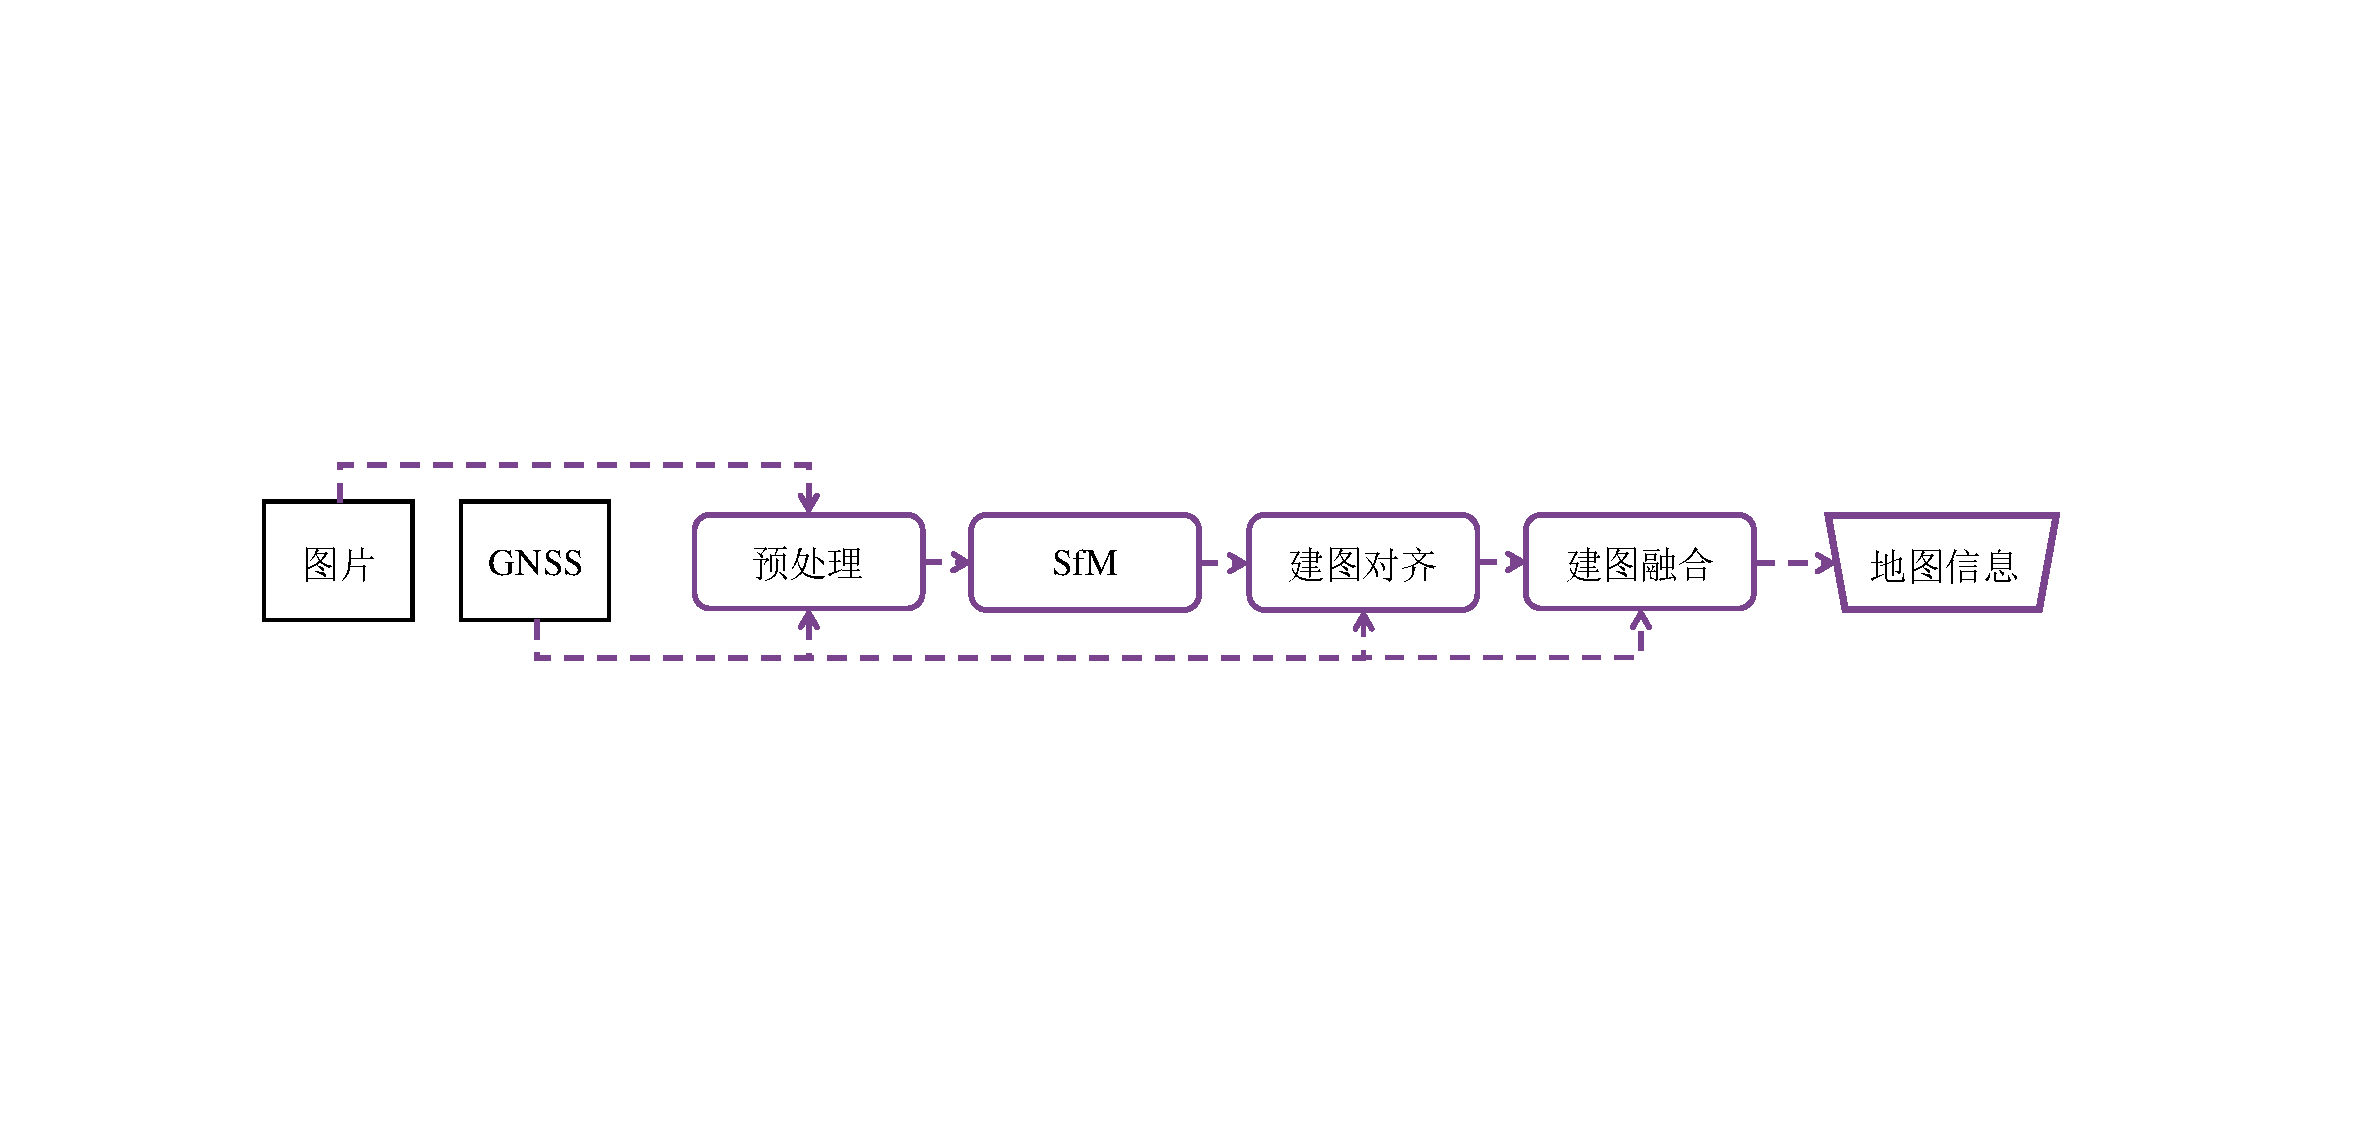
\includegraphics[width=1.0\linewidth]{mapping.pdf}
  \caption{离线建图模块整体流程}
  \label{fig:mapping}
\end{figure}

离线建图模块的整体流程如图\ref{fig:mapping}所示:首先通过图片和GNSS信息进行预处理,主要是筛选出候选关键帧以及进行语义分割(Semantic Segmentation)等操作;紧接着纯图像首先进行SfM以获得在视觉建图世界坐标系下的相机位姿和地图点云;然后使用GNSS信息和SfM结果进行建图对齐,即实现视觉建图世界坐标系和全局坐标系的对齐;此后进行建图融合,以非线性优化的方式同时优化视觉重投影误差和GNSS提供的位置误差;最后输出分层次的的地图。

值得注意的是,在建图阶段本文并没有使用到惯性信息,这主要由于惯性信息的使用必须同时满足“时间连续”和“时间间隔合理”两个条件才可以获得较好的效果,否则,不连续的时间会导致积分中断,过长的时间间隔会导致积分误差过大,而本文所假设的建图情况并不一定同时满足上述两个条件,故而只使用图片和GNSS信息。

\section{建图预处理}
预处理部分的主要目的是提高建图的效率并准备好建图所需数据,具体工作是根据图像和GNSS信息筛选出候选关键帧并根据建图需求对图片进行一系列处理,包括语义分割、特征提取和特征匹配。

\subsection{候选关键帧筛选}
在建图过程中,关键帧的选择对于建图效率和精度有着重要影响,关键帧的选择一般遵循以下的原则:(1)关键帧之间必须有足够的共视区域,这是为了保证有足够的特征点可以被匹配;(2)关键帧之间的距离不宜太小,这是为了降低重投影误差对地图点云精度的影响,如图\ref{fig:keyframe}所示,当地图点在相机2上偏移了同样一个角度$\delta \theta$时,对地图点的估计误差会因为帧间相对距离的不同而有差异,而当帧间位移较小的时候,误差明显加大。为了达成原则(1),本文使用连续的图像帧作为候选关键帧,保证了帧之间有足够的共视区域;为了达成原则(2),本文使用了GNSS提供的位置信息来过滤掉距离过近的候选关键帧,设定过滤阈值为1.5m,即如果两个候选关键帧之间的距离小于1.5m,则保留其中一个,否则保留两者。

\begin{figure}
  \centering
  \begin{tikzpicture}[x=0.75pt,y=0.75pt,yscale=-1,xscale=1]
  %uncomment if require: \path (0,300); %set diagram left start at 0, and has height of 300

  %Straight Lines [id:da9271411216933381] 
  \draw    (92,141) -- (134,15) ;
  \draw [shift={(92,141)}, rotate = 288.43] [color={rgb, 255:red, 0; green, 0; blue, 0 }  ][fill={rgb, 255:red, 0; green, 0; blue, 0 }  ][line width=0.75]      (0, 0) circle [x radius= 3.35, y radius= 3.35]   ;
  %Straight Lines [id:da29003793579323167] 
  \draw    (92,141) -- (156,141) ;
  \draw [shift={(159,141)}, rotate = 180] [fill={rgb, 255:red, 0; green, 0; blue, 0 }  ][line width=0.08]  [draw opacity=0] (10.72,-5.15) -- (0,0) -- (10.72,5.15) -- (7.12,0) -- cycle    ;
  %Straight Lines [id:da5112353172737918] 
  \draw    (125,14) -- (159,141) ;
  \draw [shift={(159,141)}, rotate = 75.01] [color={rgb, 255:red, 0; green, 0; blue, 0 }  ][fill={rgb, 255:red, 0; green, 0; blue, 0 }  ][line width=0.75]      (0, 0) circle [x radius= 3.35, y radius= 3.35]   ;
  %Shape: Circle [id:dp1662355167840721] 
  \draw  [fill={rgb, 255:red, 0; green, 0; blue, 0 }  ,fill opacity=1 ] (124,30) .. controls (124,27.24) and (126.24,25) .. (129,25) .. controls (131.76,25) and (134,27.24) .. (134,30) .. controls (134,32.76) and (131.76,35) .. (129,35) .. controls (126.24,35) and (124,32.76) .. (124,30) -- cycle ;
  %Straight Lines [id:da6367497127041384] 
  \draw  [dash pattern={on 4.5pt off 4.5pt}]  (98,31) -- (159,141) ;
  %Straight Lines [id:da03601324600093769] 
  \draw    (139,104) -- (148,99) ;
  %Straight Lines [id:da9735029157865975] 
  \draw    (279,141) -- (336,17) ;
  \draw [shift={(279,141)}, rotate = 294.69] [color={rgb, 255:red, 0; green, 0; blue, 0 }  ][fill={rgb, 255:red, 0; green, 0; blue, 0 }  ][line width=0.75]      (0, 0) circle [x radius= 3.35, y radius= 3.35]   ;
  %Straight Lines [id:da52354703700931] 
  \draw    (279,141) -- (428,141) ;
  \draw [shift={(431,141)}, rotate = 180] [fill={rgb, 255:red, 0; green, 0; blue, 0 }  ][line width=0.08]  [draw opacity=0] (10.72,-5.15) -- (0,0) -- (10.72,5.15) -- (7.12,0) -- cycle    ;
  %Straight Lines [id:da9759107264201796] 
  \draw    (312,14) -- (431,141) ;
  \draw [shift={(431,141)}, rotate = 46.86] [color={rgb, 255:red, 0; green, 0; blue, 0 }  ][fill={rgb, 255:red, 0; green, 0; blue, 0 }  ][line width=0.75]      (0, 0) circle [x radius= 3.35, y radius= 3.35]   ;
  %Shape: Circle [id:dp7881999863696054] 
  \draw  [fill={rgb, 255:red, 0; green, 0; blue, 0 }  ,fill opacity=1 ] (324,33) .. controls (324,30.24) and (326.24,28) .. (329,28) .. controls (331.76,28) and (334,30.24) .. (334,33) .. controls (334,35.76) and (331.76,38) .. (329,38) .. controls (326.24,38) and (324,35.76) .. (324,33) -- cycle ;
  %Straight Lines [id:da010281824834210473] 
  \draw  [dash pattern={on 4.5pt off 4.5pt}]  (299,46) -- (431,141) ;
  %Straight Lines [id:da5937501580461493] 
  \draw    (381,104) -- (390,97) ;
  %Straight Lines [id:da707089378321986] 
  \draw [color={rgb, 255:red, 155; green, 155; blue, 155 }  ,draw opacity=1 ] [dash pattern={on 4.5pt off 4.5pt}]  (70,141) -- (466,141) ;

  % Text Node
  \draw (70,148) node [anchor=north west][inner sep=0.75pt]   [align=left] {相机1};
  % Text Node
  \draw (148,148) node [anchor=north west][inner sep=0.75pt]   [align=left] {相机2};
  % Text Node
  \draw (136,18) node [anchor=north west][inner sep=0.75pt]   [align=left] {地图点P};
  % Text Node
  \draw (150,88.4) node [anchor=north west][inner sep=0.75pt]  [font=\footnotesize]  {$\delta \theta $};
  % Text Node
  \draw (86,13.4) node [anchor=north west][inner sep=0.75pt]  [font=\footnotesize]  {$\delta d$};
  % Text Node
  \draw (257,148) node [anchor=north west][inner sep=0.75pt]   [align=left] {相机1};
  % Text Node
  \draw (415,147) node [anchor=north west][inner sep=0.75pt]   [align=left] {相机2};
  % Text Node
  \draw (351,20) node [anchor=north west][inner sep=0.75pt]   [align=left] {地图点P};
  % Text Node
  \draw (393,84.4) node [anchor=north west][inner sep=0.75pt]  [font=\footnotesize]  {$\delta \theta $};
  % Text Node
  \draw (294,30.4) node [anchor=north west][inner sep=0.75pt]  [font=\footnotesize]  {$\delta d$};
  % Text Node
  \draw (123,122.4) node [anchor=north west][inner sep=0.75pt]    {$t$};
  % Text Node
  \draw (335,122.4) node [anchor=north west][inner sep=0.75pt]    {$t$};


  \end{tikzpicture}
  \caption{关键帧之间的距离会影响地图点精度}
  \label{fig:keyframe}
\end{figure}

\subsection{语义分割}

在候选关键帧筛选之后,接下来是对图片进行语义分割。语义分割可以利用图片中的高层语义分析,协助达成SfM的静态环境假设,即SfM所重建出来的地图点云应归属于静态物体。在实际的道路建图中,这一条件的达成并不容易,例如在城市环境下,建筑物是理想的建图元素,因为其位置相对固定,短时间内外观变化较小,但是汽车、行人等元素则不适合作为建图元素,因为其位置可能变化,并且处于移动状态会使得不同时刻的相机观测不满足静态假设。因此,本文使用语义分割算法对图片进行处理,将图片中动态物体剔除,保留静态部分以便建立更加稳定和精确的地图。

\begin{table}
  \centering
  \caption{语义分割类别分布与屏蔽情况}
  \begin{tabular}{cccccccccccc}
  \toprule
  类别 & road & $\dots$ & sky & person & rider & car & truck & bus & train & motorcycle & bicycle \\
  \midrule
  标签序号 & 0    &  $\dots$ & 10  & 11 & 12 & 13 & 14 & 15  & 16 & 17 & 18 \\
  屏蔽   &     &    &    & \checkmark &  \checkmark    &  \checkmark  &  \checkmark &  \checkmark  &   \checkmark   &  \checkmark  & \checkmark \\ 
  \bottomrule 
  \end{tabular}
  \label{tab:seg}
\end{table}

因为语义分割技术只是离线建图工作中的一小部分,所以本文选择了开箱即用的语义分割模型,并根据建图模块的实际需求进行了微调。本文所选择的语义分割模型是SegFormer\cite{xie2021segformer},SegFormer是一个基于Transformer的语义分割模型,凭借其紧凑但高效的网络结构,其在语义分割精度和速度上均取得了较好的效果。本文使用了SegFormer的B1型,即SegFormer-B1在cityscapes\cite{Cordts2016Cityscapes}数据集上的预训练权重作为初始,在该数据集的灰度图像上进行了微调。cityscapes数据集是一个城市道路环境下的语义分割数据集,包含了大量的城市道路图片和对应的标签,标签中包含了道路、建筑、树木等静态物体的信息,以及汽车、行人等动态物体。微调以$1024 \times 1024$的分辨率进行了160,000轮迭代,使得模型在灰度图上的表现接近了其在彩色图片上的表现,以便在建图过程中适应建图所使用的灰度图像输入。

\begin{figure}
  \centering
  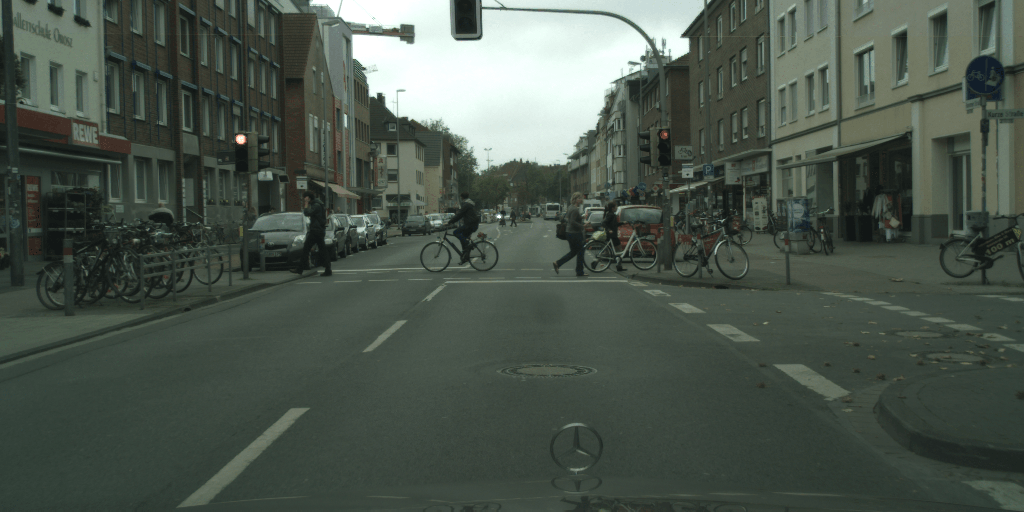
\includegraphics[width=0.47\linewidth]{seg.png}
  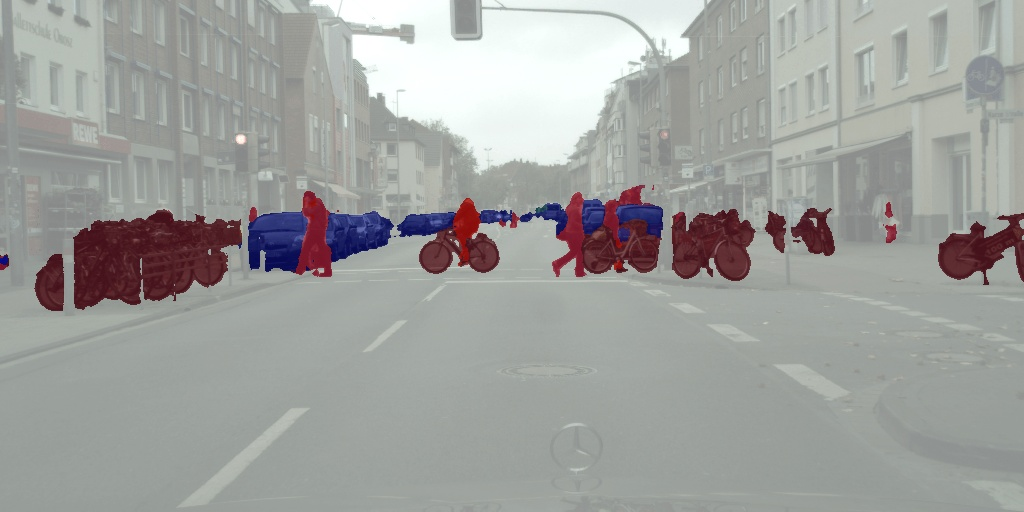
\includegraphics[width=0.47\linewidth]{seged.jpg}
  \caption{语义分割效果}
  \label{fig:seg}
\end{figure}

本文的语义分割模型在cityscapes数据集上训练,其输出的类别以及每一类别的标签序号如表~\ref{tab:seg}所示。在建图过程中,本文会将潜在的移动物体类别所包含的像素位置标记为屏蔽,后续的特征提取和匹配过程将不考虑这些像素位置,具体的屏蔽情况也汇报在表~\ref{tab:seg}中。语义分割的实际效果以及屏蔽内容以图~\ref{fig:seg}所示,左侧为原始图像,右侧为语义分割的结果示意图,其中被白色覆盖的区域为保留部分,被其他颜色覆盖的区域为屏蔽部分,可以看到被屏蔽的大部分区域均为行人、自行车等动态物体。

\section{SfM}

经过建图预处理的图像会进行SfM,构建初步的点云地图。SfM是一种摄影测量技术,用于从二维图像序列中估计三维结构\cite{schonberger2016structure}。SfM以地图关键帧序列$\symcal{K} = \{K_i \mid i=1 \ldots N_{K} \}$和相机内参矩阵$\symbf{K}$作为输入,输出地图关键帧序列的六自由度位姿$\symcal{T} = \{\symbf{T}^{k_i}_w \mid i=1 \ldots N_K \}$以及空间点集$\symcal{P} = \{\symbf{p}_{m}^{w} \in \mathbb{R}^3 \mid m=1 \ldots N_P\}$,统称为稀疏点云结构。需要注意的是,相机内参矩阵数量本应与地图关键帧数量对应,但是对于固定路线定位来说,建图所用图像均由同一相机拍摄,因此共用一个内参。

SfM通常以特征检测和匹配为第一步:对于每个地图关键帧$K_i$,SfM检测出一组局部特征$\symcal{F}_i = \{(\symbf{x}_j, \symbf{f}_j) \mid j = 1, \ldots, N_{F_i}\}$,其中 $\symbf{x}_j \in \mathbb{R}^2$表示特征点的位置,$\symbf{f}_j \in \mathbb{R}^{d_l}$ 表示其 ${d_l}$ 维特征描述子。随后,进行图像匹配以识别捕捉到同一场景区域的关键帧,在这个过程中基于描述子的匹配方法被广泛采用。在本文中,由于建图预处理部分已经对地图关键帧的相对位置进行了筛选,因此相邻的关键帧已经具有了足够的共视区域,可以直接进行匹配,简化了匹配过程。

在相邻帧之外,为了通过闭环检测减轻漂移的问题,本文在建图时还引入了基于闭环检测的匹配方法。回环检测通过为每个关键帧提取一个$d_g$维的图像描述子$\symbf{D}_i \in \mathbb{R}^{d_g}$,并计算所有地图关键帧之间图像描述子的相似度得分来实现,得分超过预设阈值$s$的前$m$对被选为回环闭合对。对于所有匹配上的地图关键帧对,SfM通过特征点描述子匹配特征点,并利用这些匹配点估计两个关键帧的相对位姿。

在完成特征检测和匹配之后,SfM进一步估计地图关键帧的位姿以及结构的空间坐标。通过选择第一个地图关键帧作为视觉建图世界坐标系的原点,所有关键帧的位姿$\symcal{T}$都可以递归得通过相对位姿转换进行粗略估计。随后,SfM用三角化方法在视觉建图世界坐标系中估计稀疏点云结构$\symcal{P}$的粗略空间坐标。位姿估计与三角化过程密切相关:位姿的不确定性会导致三角化点的可靠性下降,反之亦然。因此,为了获得精确的 $\symcal{T}$ 和 $\symcal{P}$,更精确的优化过程必不可少。

光束法平差(Bundle Adjustment, BA)是一种高效的位姿和点云结构优化方法,可通过最小化重投影误差来同时两种参数:
\begin{equation}
\label{eq:reproj_error}
E_i = \sum_{j}\rho(\Vert \hat{\symbf{x}}_j - \pi(\symbf{T}^{k_i}_w, \symbf{p}_{m}^{w}) \Vert ^2_2),
\end{equation}
其中,$\symbf{p}_{m}^{w}$是图像特征点$\hat{\symbf{x}}_j$对应的空间点三维坐标,$\rho$是一种损失函数,用于降低异常值的权重。函数 $\pi(\cdot)$ 将空间点投影到图像空间,定义如下:
\begin{equation}
\label{eq:proj_func}
\pi(\symbf{T}^{k_i}_w, \symbf{p}_{m}^{w}) = [\symbf{K}\cdot(\symbf{R}_w^{k_i}\cdot\symbf{p}_{m}^{w}+\symbf{t}_w^{k_i})/d_j]_{0:2},
\end{equation}
其中,$d_j$ 是 $\symbf{p}_{m}^{w}$ 在相机坐标系中的深度,$[\cdot]_{0:2}$ 表示选择向量的前两个元素。需要注意的是,$E_i$ 表示单张图像的重投影误差,因此整个BA是对输入图像序列中的所有重投影误差进行累积优化的结果。BA的进行需要使用非线性优化方法,例如高斯-牛顿法或者Levenberg-Marquardt法,这需要误差函数\eqref{eq:reproj_error}关于参数$\symbf{T}^{k_i}_w$和$\symbf{p}_{m}^{w}$的雅可比矩阵,优化过程及雅可比矩阵的推导参考附录~\ref{appendix:quat}。


\section{建图对齐}

SfM可以为离线建图阶段的图像提供精化的位姿和稀疏点云地图,但这些位姿和结构并不是在全局坐标系下的,并且缺乏真实世界的物理尺度,因此不适用于实际的定位任务。为了解决这一问题,本文利用图像的对应GNSS观测数据,将SfM的输出与真实世界的物理尺度对齐。标准GNSS报文仅提供地理坐标系中的纬度、经度和海拔信息,地理坐标系是一种墨卡托坐标系,而地图关键帧位姿和点云结构都是在笛卡尔坐标系中。因此,需要首先将原始GNSS报文信息从地理坐标系统转换为笛卡尔ENU坐标系中的位置序列
$\symcal{L} = \{\symbf{l}_{k_i}^g \in \mathbb{R}^3 \mid i=1 \ldots N_K \}$。
这一过程遵循\citet{subirana2011transformations} 提出的转换方法,并设置
$\symbf{l}_{k_1}^g = \symbf{0}$ 以确保数值稳定性。

由于建图对齐过程不仅需要解决视觉建图世界坐标系与全局坐标系之间的变换问题,还需要处理两者之间的尺度差异,本课题采用三维相似变换(Similarity Transformation in 3D, Sim3)~\cite{horn1987closed}。Sim3包括一个比例因子 $s$、一个旋转矩阵 $\symbf{R}_w^g$ 和一个平移向量 $\symbf{t}_w^g$。如果第 $i$ 个地图关键帧在视觉建图世界坐标系中的位置为 $\symbf{t}_{k_i}^{w} = -{\symbf{R}_w^{c_i}}^T \cdot \symbf{t}_w^{k_i}$,对应的 GNSS 观测值为 $\symbf{l}_{k_i}^g$,则Sim3变换可以将它们对齐,具体如下:
\begin{equation}
    \symbf{l}_{k_i}^g = s \cdot \symbf{R}_w^g \cdot \symbf{t}_{k_i}^{w} + \symbf{t}_w^g.
\end{equation}
Sim3 参数的最小二乘解可以通过求解以下优化问题获得:
\begin{equation}
  s^*, {\symbf{R}_w^g}^*, {\symbf{t}_w^g}^* = \underset{s,\symbf{R}_w^g,\symbf{t}_w^g}{\text{arg min}} \sum_i^{N_I} \Vert \symbf{l}_{k_i}^g - s \cdot \symbf{R}_w^g \cdot \symbf{t}_{k_i}^{w} - \symbf{t}_w^g \Vert_2^2.
\end{equation}

利用 Sim3 参数,可以方便地将地图关键帧位姿 $\symcal{T}$ 和稀疏点云结构 $\symcal{P}$ 转换到具有真实物理尺度的全局坐标系中:
\begin{equation}
\begin{cases}
    \symbf{R}^{k_i}_g = {\symbf{R}^{k_i}_{w}} \cdot {\symbf{R}_w^g}^{-1}, \\
    \symbf{t}^{k_i}_g = s \cdot \symbf{t}_w^{c_i} - {\symbf{R}^{k_i}_{w}} \cdot {\symbf{R}^{g}_{w}}^{-1} \symbf{t}_w^g, \\
    \symbf{p}_m^g = s \cdot \symbf{R}_w^g \cdot \symbf{p}_{m}^{w} + \symbf{t}_w^g,
\end{cases}.
\end{equation}

\section{建图融合}

尽管已经获得了较为精确的地团关键帧位姿和稀疏点云结构,并成功将它们转换到全局坐标系中,但在求解Sim3参数的最小二乘解时仍可能引入误差。为了获得更精确的位姿和点云结构,还需要将当前的全局坐标系参数与GNSS观测进行融合优化。该融合过程需要确保地图关键帧位姿和点云结构同时满足GNSS和视觉的观测,因此需要在视觉BA的基础上融合进GNSS的观测约束,将全局坐标系中的重投影误差重新表示为:
\begin{equation}
\label{eq:new_reproj}
    E_i = \sum_{j}\rho\left(\Vert \symbf{x}_j - \pi(\symbf{T}^{k_i}_g, \symbf{p}_{m}^{g}) \Vert ^2_2\right) 
    + \alpha \cdot \rho\left(\Vert -\symbf{R}_g^{k_i^T}\cdot\symbf{t}_g^{k_i} - \symbf{l}_{k_i}^g \Vert_2^2\right),
\end{equation}
其中,$\alpha$ 是一个权重系数,用于平衡视觉重投影误差与位置偏差。然后通过BA过程对式 \eqref{eq:new_reproj} 中的误差进行最小化。

至此,已经介绍了地图关键帧位姿和稀疏点云结构的优化,这些空间信息有效地描述了环境结构。然而,为了在定位过程中充分利用这些信息,还需要视觉地图关键帧描述子和稀疏点云的描述子,用于地图与实时捕获图像之间的匹配。在离线建图过程中,直接使用 $\{\symcal{F}_i \mid i = 1, \ldots, N_K\}$ 作为地图点的描述子,$\{\symbf{D}_i \mid i = 1, \ldots, N_K\}$ 作为关键帧描述符。离线建图模块的最终输出可以分为两个层级:粗粒度层级和细粒度层级。粗粒度层级输出包括关键帧位姿和描述符,用于建立图像匹配关系;而细粒度层级输出包括点描述符和点结构,用于实现点的匹配。

\section{本章总结}
本章主要介绍了固定路线定位系统的整体架构和离线建图模块的设计。整体架构中建图与定位以异构的形式存在,即建图以SfM技术为基础,而定位以SLAM技术为基础,这种异构设计能够充分发挥SfM的精度优势和SLAM的速度优势。离线建图模块以视觉和GNSS融合的SfM为基础,同时根据建图需求引入了基于深度学习的语义分割、回环检测以及特征点提取技术,将更多的人类经验加入到离线建图中。离线建图模块的另一个特点是在传统SfM的基础上引入了GNSS观测作为约束和融合信息,这能够显著提升建图的精度。
